\documentclass[a4paper, 12pt]{article}%тип документа

%отступы
\usepackage[left=1.5cm,right=1cm,top=2cm,bottom=3cm,bindingoffset=0cm]{geometry}
\setlength{\parindent}{5ex}

%Русский язык
\usepackage[T2A]{fontenc} %кодировка
\usepackage[utf8]{inputenc} %кодировка исходного кода
\usepackage[english,russian]{babel} %локализация и переносы

%Вставка картинок
\usepackage{graphicx}
\graphicspath{{pictures/}}
\DeclareGraphicsExtensions{.pdf,.png,.jpg,}
\usepackage{wrapfig}

%Графики
\usepackage{pgfplots}
\pgfplotsset{compat=1.9}

%Математика
\usepackage{amsmath, amsfonts, amssymb, amsthm, mathtools}

%Таблицы
\usepackage{longtable} 
\usepackage{float}

%Римские цифры
\newcommand{\RomanNumeralCaps}[1]{\uppercase\expandafter{\romannumeral#1}}

\usepackage{multirow}


\begin{document}
	\begin{titlepage}
		\begin{center}
			\textsc{Федеральное государственное автономное образовательное учреждение высшего образования«Московский физико-технический институт (национальный исследовательский университет)»\\[5mm]
			}
			
			\vfill
			
			\textbf{Лабораторная работа: \\[3mm]
				Фурье спектроскопия
				\\[50mm]
			}
			
		\end{center}
		
		\hfill
		\begin{minipage}{.5\textwidth}
			Выполнили студенты:\\[2mm]
			Сериков Василий Романович\\[2mm]
			Группа: Б03-102\\[5mm]
			Сериков Алексей Романович\\[2mm]
			Группа: Б03-102\\[5mm]
			
		\end{minipage}
		\vfill
		\begin{center}
			Москва, 2024 г.
		\end{center}
		
	\end{titlepage}
	
	\newpage
	\textbf{Аннотация}\\
	
	Ознакомление с принципами работы Фурье-спектрометров, цифровой обработкой оптических сигналов, поглощением света оптическими средами, с колебательно-вращательными спектрами молекул. \\
	
	\textbf{Теоретические сведения: }\\
	
	
	Аппаратная функция спектрального прибора - это его отклик на монохроматическую световую волну.
	
	Поэтому рассмотрим форму спектра на входе Фурье-спектрометра, когда на его вход поступает плоская монохроматическая волна, распространяющаяся вдоль оптической оси прибора. Запишем $E(t)$ в виде
	$$
	E(t)=E_0 \cos \omega_0 t .
	$$
	
	Корреляционная функция этого сигнала запишется следующим образом:
	$$
	R(\tau)=E_0^2 \overline{\cos \omega_0 \tau \cdot \cos \omega_0(t-\tau)}=\frac{1}{2} \cos \omega_0 \tau .
	$$
	
	Далее находим общее выражение для спектра:
	$$
	G(\omega)=\frac{1}{2} \int_0^{\infty} \cos \omega_0 \tau \cos \omega \tau \alpha t .
	$$
	
	Это выражение даст нам одну монохроматическую линию на частоте $\omega_0$. Однако в реальном Фурье-спектрометре корреляционная функция записывается за конечное время, которое ограничивается максимальной разностью хода в интерферометре $\Delta_{\boldsymbol{n}}$. Поэтому 
	$$
	\begin{aligned}
		& G(\omega)=\frac{E_0^2}{2} \int_0^{\Delta_0 / c} \cos \omega_0 \tau \cos \omega \tau c \hbar= \\
		& =\frac{E_0^2}{4} \int_0^{\Delta_{-} / c}\left[\cos \left(\omega_0-\omega\right) \tau+\cos \left(\omega_0+\omega\right) \tau\right] d \tau= \\
		& =\frac{E_0^2 c}{4 \Delta_{-}}\left[\operatorname{sinc}\left(\omega_0-\omega\right) \frac{\Delta_{-}}{c}+\sin \left(\omega_0+\omega\right) \frac{\Delta_m}{c}\right] .
	\end{aligned}
	$$
	
	Здесь функция $\operatorname{sinc}(x)=\sin x / x$.
	Член $\operatorname{sinc}\left[\left(\omega_0+\omega\right) \Delta_{-} / c\right]$ выражения в области частот $\omega>0$ дает незначительный вклад, и им в дальнейшем место пренебречь. В результате аппаратная функция Фурье-спектрометра может быть представлена в виде
	$$
	A(v)=\frac{E_0^2 c}{4 \Delta_a} \sin c\left[2 \pi\left(v_0-v\right) \frac{\Delta_E}{c}\right] .
	$$
	
	Первый минимум этой функции будет, когда
	$$
	2\left(v_0-v\right) \frac{\Delta_t}{c}=1 \text {, }
	$$
	
	или при
	$$
	\delta v=v_0-v=\frac{c}{2 \Delta_n} .
	$$
	
	Отсюда в соответствии с критерием Рэлея разрешающая сила есть
	$$
	R =\frac{2 v \Delta_e}{c}=\frac{2 \Delta_n}{\lambda}
	$$
	
	
	При поступлении в интерферометр излучении от источника яркостью $B(v)$ со сложным спектральным составом зависимость светового потока на выходе прибора от разности хода $\Delta$ примет вид
	$$
	\begin{aligned}
		& \Phi(\Delta)=q \int_0^{\infty} B(v) \cos \left(2 \pi v \frac{\Delta}{c}\right) d v= \\
		& =q \int_0^{\infty} B(v) d v+q \int_0^{\infty} B(v) \cos \left(2 \pi v \frac{\Delta}{c}\right) d v .
	\end{aligned}
	$$
	
	Пусть одно из зеркал будет двигаться равномерно со скоростью $v$. Тогда $\Delta=v t$, и второй член выражения примет вид
	$$
	\Phi(t)=q \int_0^{\infty} B(v) \cos \left(2 \pi v \frac{v}{c} t\right) d v .
	$$
	
	Если положить
	$$
	B(v)=B(-v),
	$$
	
	то подынтегральная функция будет четной, и тогда
	$$
	\Phi(t)=\frac{q}{2} \int_{-\infty}^{\infty} B(v) \cos \left(2 \pi v \frac{v}{c}\right) d .
	$$
	
	\textbf{Экспериментальная установка:}\\
	
	 Измерения выполняются на приборе Varion 3100, который представляет собой стационарный настольный прибор, состоящий из
	двух лучевого интерферометра, источника, приемника излучения,
	оптической системы и блока электроники.
	\par В нем применяются сменные фотоприемники и светоделители,
	что позволяет использовать прибор для измерения спектров пропускания и поглощения в широком диапазоне ИК-излучения. Он разбит
	на под диапазоны: 16000 — 3000 см и 7000 - 400 см. Разрешение
	прибора может изменяться от 16 см до 0,25 см. В работе используются стандартные кюветы, заполненные различными газами. Они
	попеременно помещаются оператором в специальный отсек для образцов. Управление прибором, регистрация и обработка спектра
	осуществляются компьютером. 
	
	
	\begin{figure}[H]
		\centering
		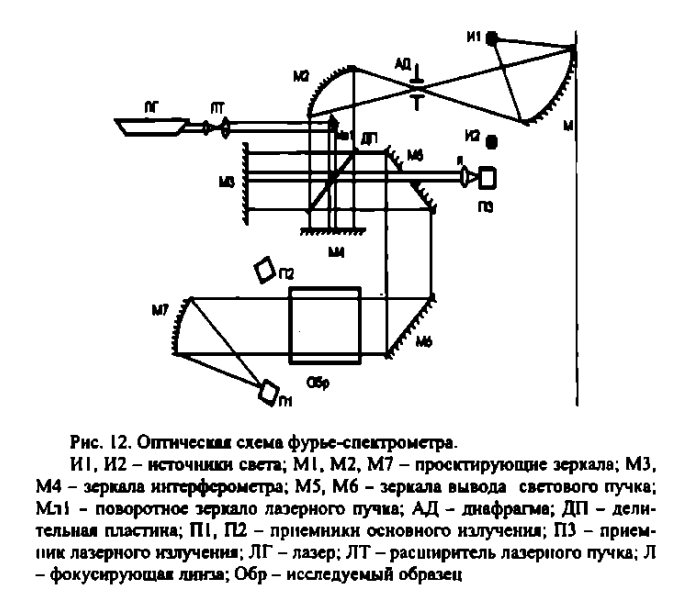
\includegraphics[width=1\linewidth]{ust}
		\caption{Экспериментальная установка}
	\end{figure}
	
	\textbf{Ход работы:}\\
	
	1) Были произведены попытки измерения спектров поглощения газов: $CO$, $C_2H_2$, $NH_3$, $CH_4$\\
	
	
	
	
	
	
	\end{document}